\section{Retrieval Performance}\label{sec:retrieval-performance}
In the following sections, we are going to describe the methods and present the results of the experiments we used to assess the performance of the system.
In this first part of the evaluation, we used several different formulas to evaluate the system.
Moreover, we carried out two different types of experiments to test several different aspects of our information retrieval system.

\subsection{Needles in a Haystack}\label{subsec:needles-in-a-haystack}
In this first batch of experiments, we wanted to test the accuracy of the system's document retrieval.
Since the system contains almost one million documents (the haystack), it is very difficult to know the precise number of relevant documents for each user query -- the number of relevant documents is needed for the computation of both the recall and the F1 score (Section~\ref{subsec:evaluation-methods}).
For this reason, we decided to imagine four different queries, and for each one of them, we created four different API specifications (the needles).
By doing so, we know the number of relevant documents per query -- four in this case -- and we can check how many the system is able to retrieve. \\ \\
Initially, we ran this experiment on four different queries, and for each query, we used ChatGPT 3.5 \footnote{https://chatgpt.com/} to help us generate valid random API specifications related to that query.
The generated specifications can be found in our repository \footnote{https://github.com/APIScout/evaluation} in the \verb|needles| directory.
The result of this experiment can be found in Figure~\ref{fig:nh-1}.
In Table~\ref{tab:metrics-prf}, we have the overall score for each metric (Equation~\ref{eq:overall}) for each $@K$.

\begin{table}[!h]
    \begin{center}
        \begin{tabular}{l c c c c c c c c c c}
            \hline
            \textbf{Metric} & \textbf{@1} & \textbf{@2} & \textbf{@3} & \textbf{@4} & \textbf{@5} & \textbf{@6} & \textbf{@7} & \textbf{@8} & \textbf{@9} & \textbf{@10} \\ \hline
            $\overline{\text{Precision}}$ & 1.0 & 1.0 & 1.0 & 0.81 & 0.65 & 0.58 & 0.5 & 0.47 & 0.42 & 0.37 \\
            $\overline{\text{Recall}}$ & 0.25 & 0.5 & 0.75 & 0.81 & 0.81 & 0.87 & 0.87 & 0.94 & 0.93 & 0.93 \\
            $\overline{\text{F1 Score}}$ & 0.4 & 0.67 & 0.86 & 0.81 & 0.72 & 0.7 & 0.64 & 0.65 & 0.58 & 0.53 \\ \hline
        \end{tabular}
    \end{center}

    \caption{Mean score for each metric $@K$ for Figure~\ref{fig:nh-1}}
    \label{tab:metrics-prf}
\end{table}

\noindent In addition to this experiment, we also tried to see if the length of the query would impact the retrieval performance of the system.
To test this, we took the query -- for example \("\)weather forecast service\("\) -- and created four sub-queries.
The generated sub-queries would be, in this case, \("\)weather\("\), \("\)weather forecast\("\), and \("\)weather forecast service\("\).
The fourth one, however, is a random substring taken from one of the natural language tags of the specification.
For example, \("\)the API returns the next 4 days of weather forecasts\("\).
This second experiment using subqueries was done on each one of the original four queries, generating the graphs in Figures~\ref{fig:nh-2},~\ref{fig:nh-3},~\ref{fig:nh-4}, and~\ref{fig:nh-5}.
In addition to these graphs, we have also generated a t-SNE plot (Section~\ref{subsec:t-sne-plots}) for each group of subqueries.
These plots can be found in Figures~\ref{fig:tsne-2},~\ref{fig:tsne-3},~\ref{fig:tsne-4}, and~\ref{fig:tsne-5}.

\begin{figure}[!h]
    \begin{center}
        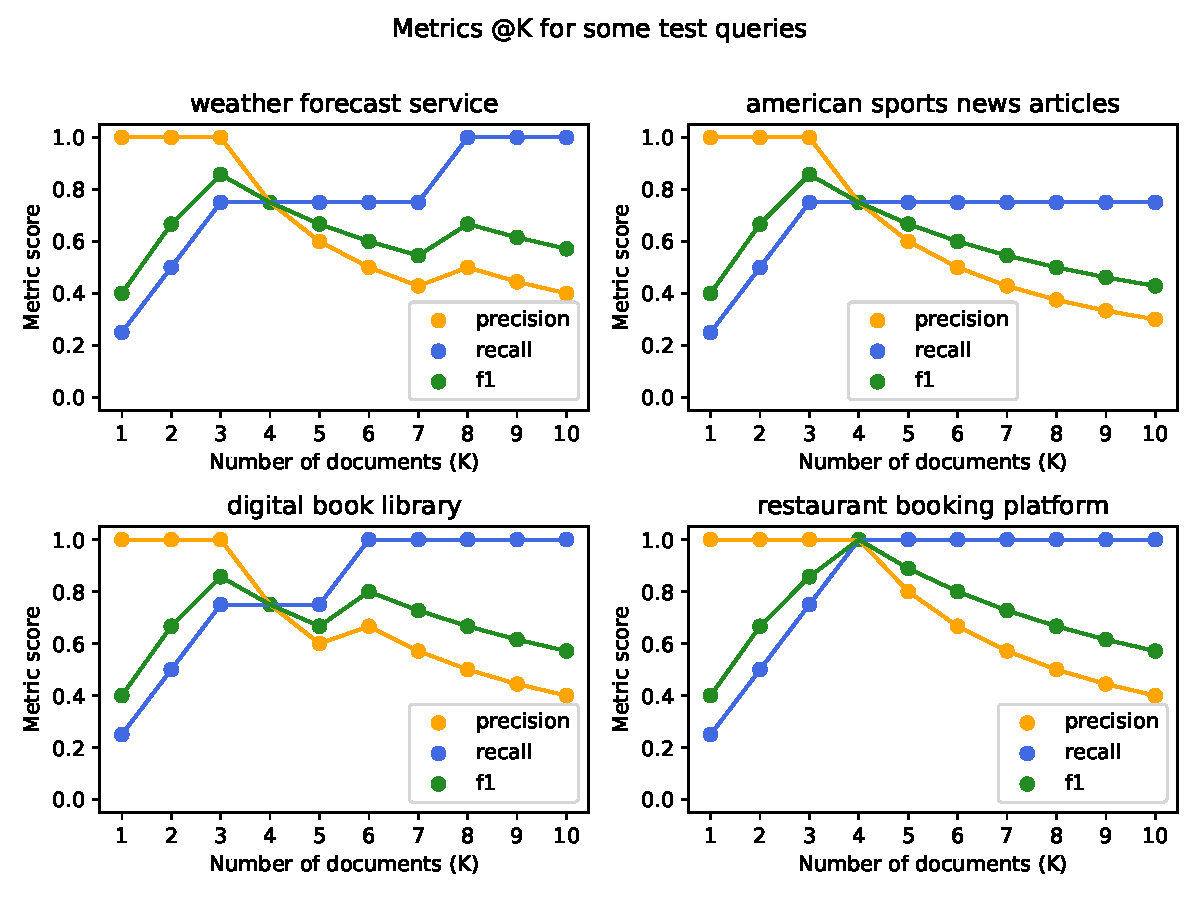
\includegraphics[width=0.8\linewidth]{assets/pdf/evaluation/prec-rec-queries}
    \end{center}

    \caption{Needles in a haystack experiment on four random queries}
    \label{fig:nh-1}
\end{figure}

\noindent To further analyze the results of this batch of experiments, we would like to understand if a high value of the parameter $K$ and a small query containing only keywords are causally related to a high recall. \\ \\
To verify this causation, we first need to define all of its nodes.
Since we are dealing with four \("\)needles\("\) (inserted documents), we define a high $K$ to be $K\geq3$ and the precision to be $P\geq0.75$.
Finally, we define a small query to have a number of words $w$ to be $w\leq4$.
Moreover, in this last case, we consider $K$ to be 10.
From all these elements, we can build our causal graph (Figure~\ref{fig:dag-1}).

\begin{figure}[!h]
    \begin{center}
        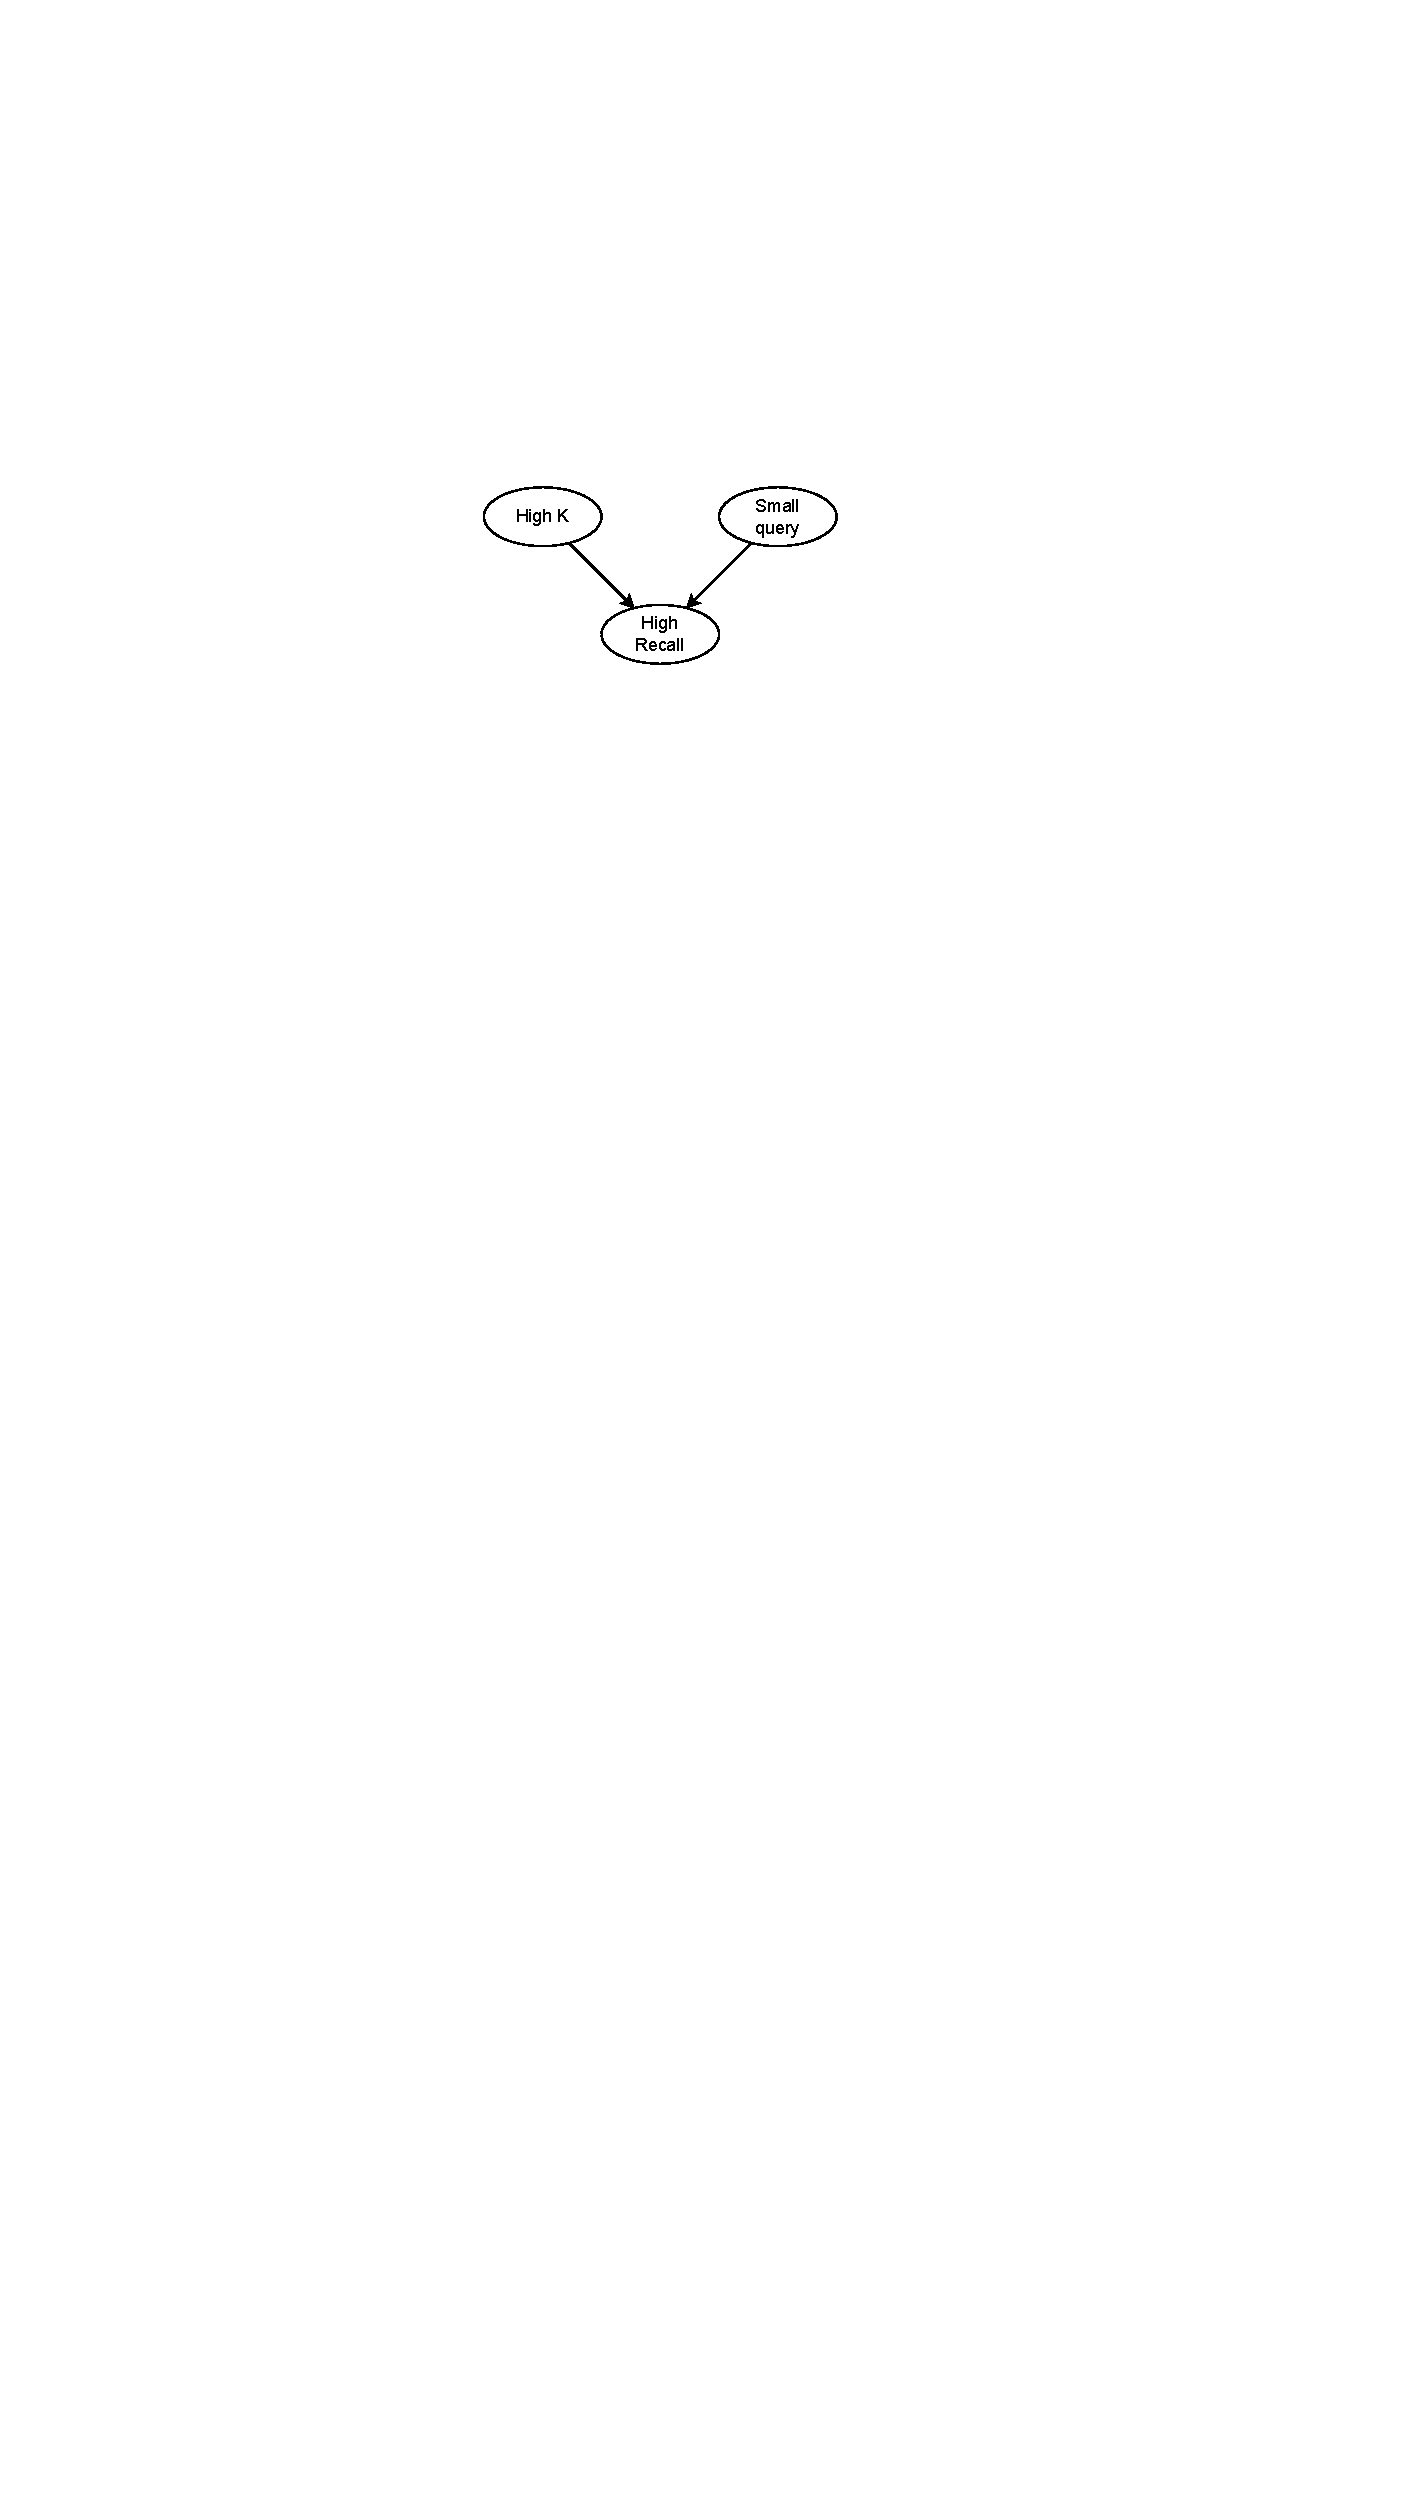
\includegraphics[width=0.3\linewidth]{assets/pdf/evaluation/dag-rec}
    \end{center}

    \caption{Causal graph}
    \label{fig:dag-1}
\end{figure}

\noindent Now that we have built the causal graph, we would like to compute the probability that each relation (an edge in the graph) is a causal relation.
To do so, we define that the probability must be computed by using Equation~\ref{eq:prob}.

\begin{equation}
    P_i = \frac{\text{Cases matching the restrictions}}{\text{Cases that should match the restrictions}}
    \label{eq:prob}
\end{equation}

\noindent With the probability formula defined, we can now proceed to compute the probabilities for each path.
In the case of the path $\text{High $K$} \rightarrow \text{High Recall}$, we have a probability of:
\[P_1 = \frac{14}{20} = 0.7\]
In the case of the path $\text{Small Query} \rightarrow \text{High Recall}$, we have a probability of:
\[P_2 = \frac{15}{16} = 0.9\]
The final causal graph can be found in Figure~\ref{fig:rec-probs}.
In this graph, we can see that there are very high probabilities that a high value of $K$ or a small query will lead to a high recall.

\begin{figure}[!h]
    \begin{center}
        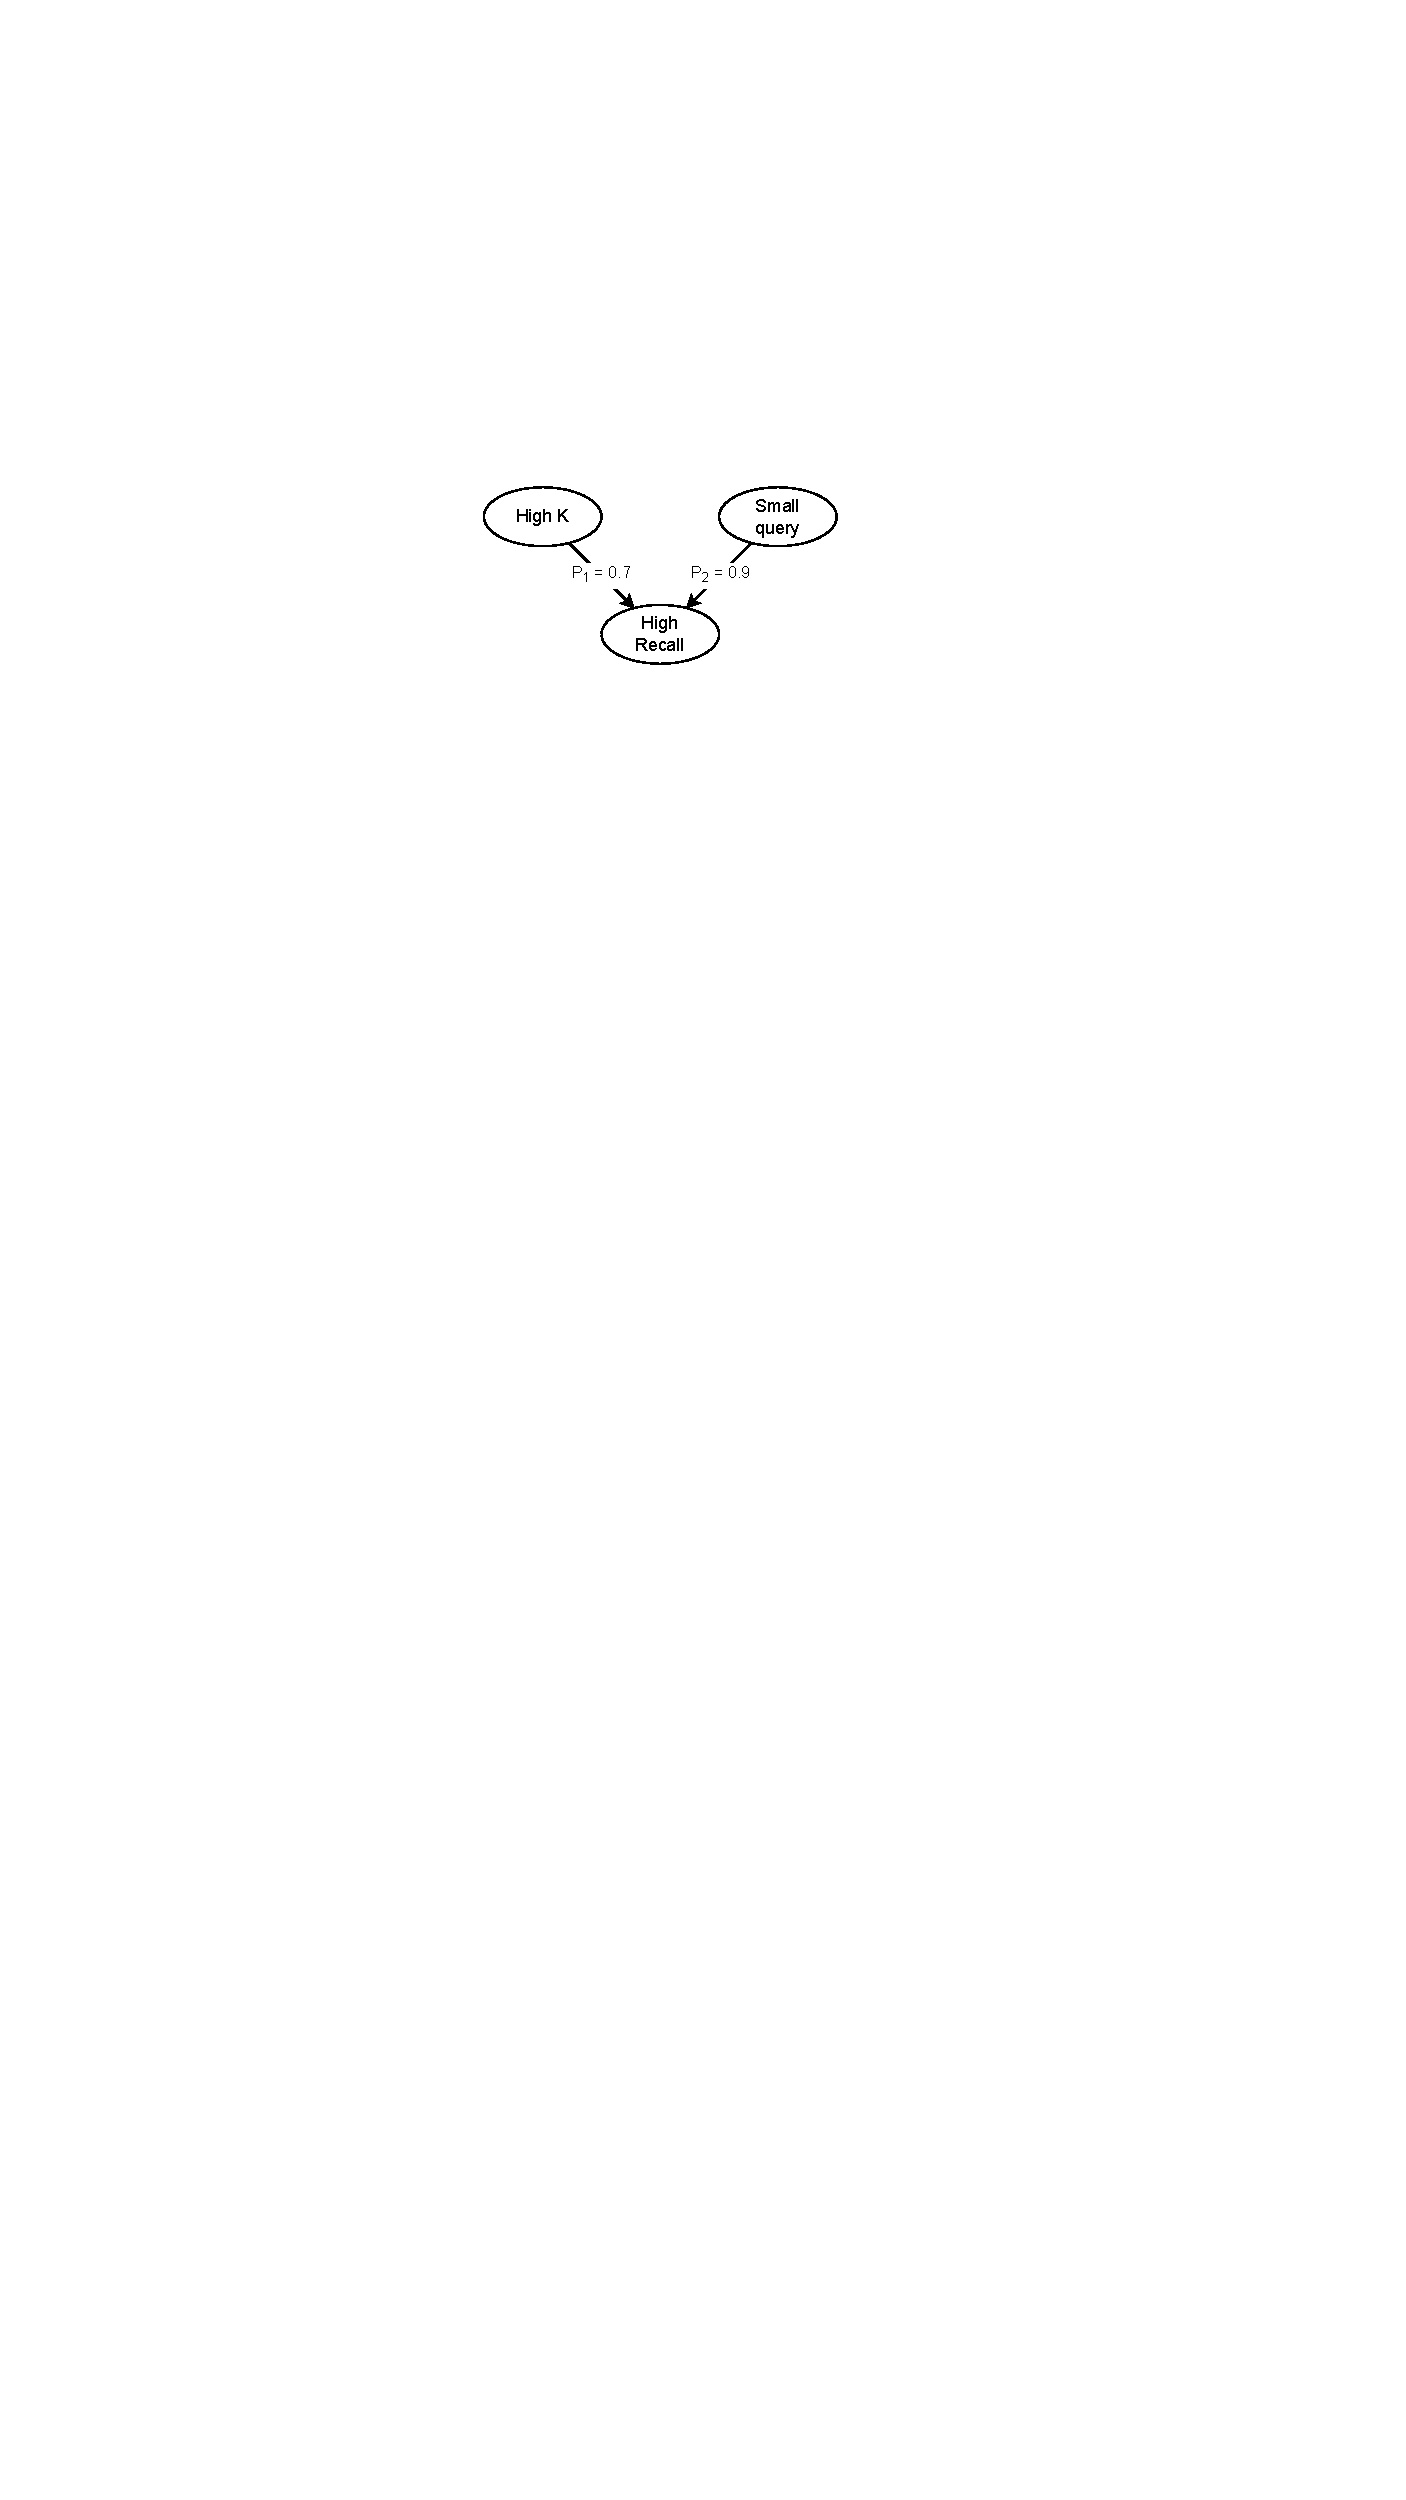
\includegraphics[width=0.3\linewidth]{assets/pdf/evaluation/dag-rec-probs}
    \end{center}

    \caption{Causal graph with probabilities}
    \label{fig:rec-probs}
\end{figure}

% ===========================================
% ===========================================

\begin{figure}[!h]
    \begin{center}
        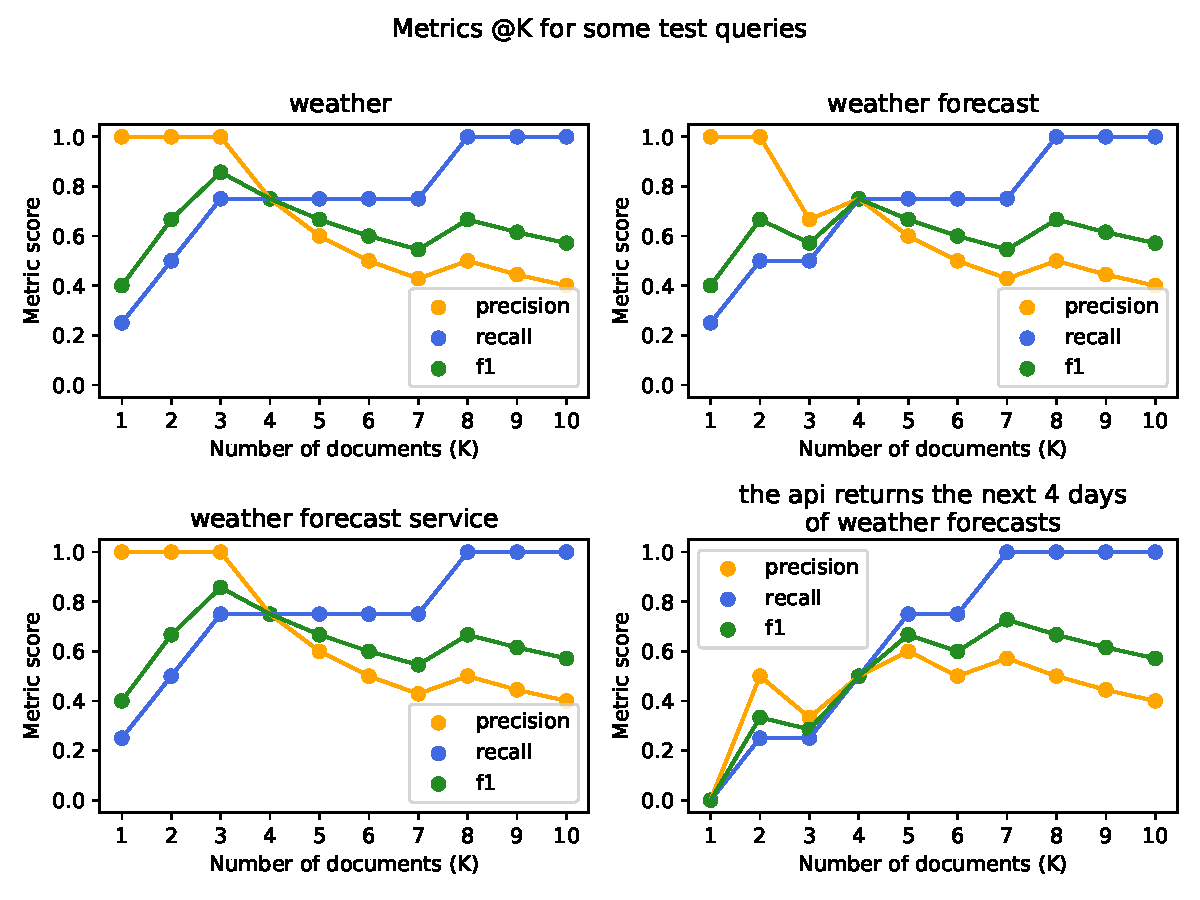
\includegraphics[width=0.8\linewidth]{assets/pdf/evaluation/prec-rec-weather}
    \end{center}

    \caption{Needles in a haystack experiment on different length queries related to weather forecast}
    \label{fig:nh-2}
\end{figure}

\begin{figure}[!h]
    \begin{center}
        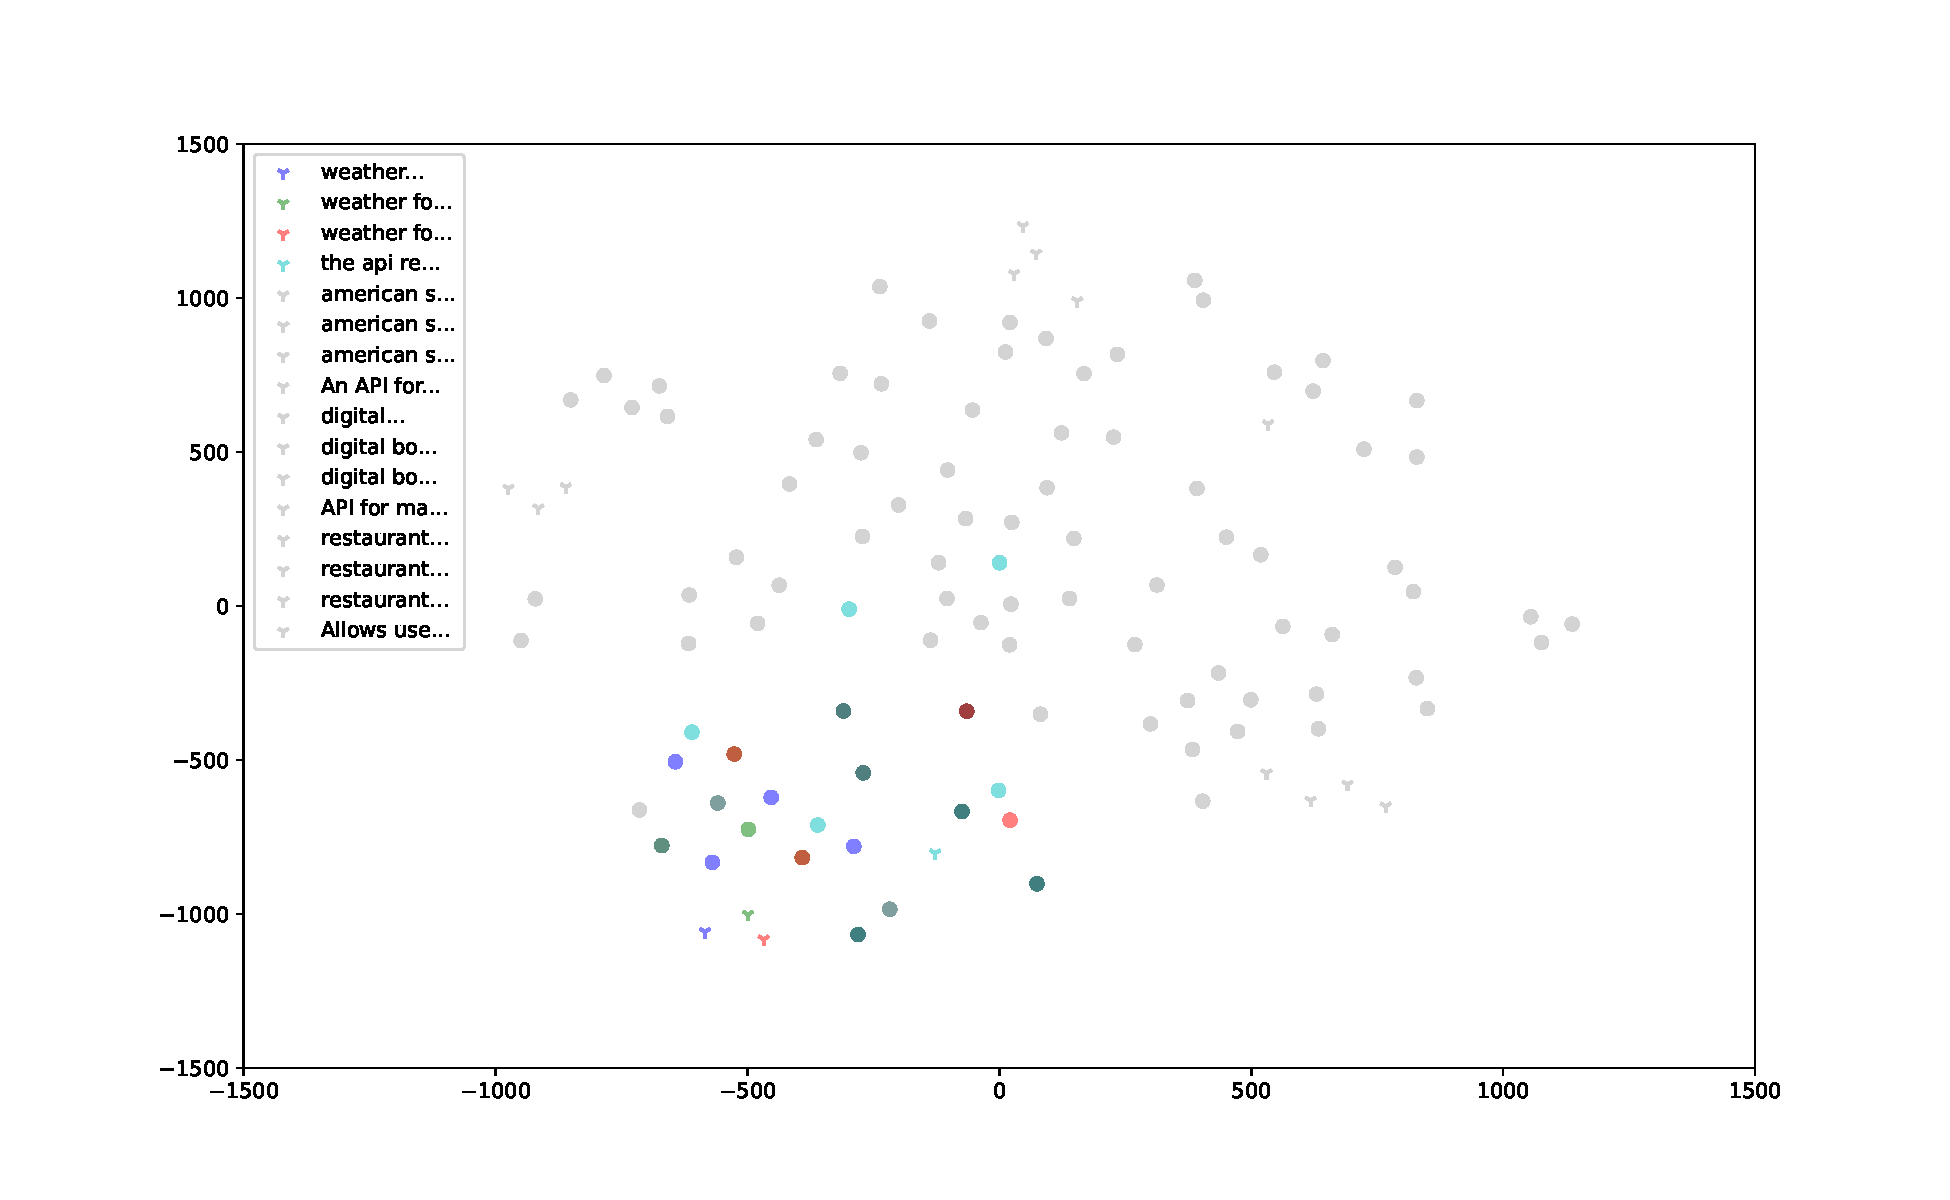
\includegraphics[width=0.8\linewidth]{assets/pdf/evaluation/tsne-weather}
    \end{center}

    \caption{t-SNE graph for the weather forecast queries}
    \label{fig:tsne-2}
\end{figure}

% ===========================================
% ===========================================

\begin{figure}[!h]
    \begin{center}
        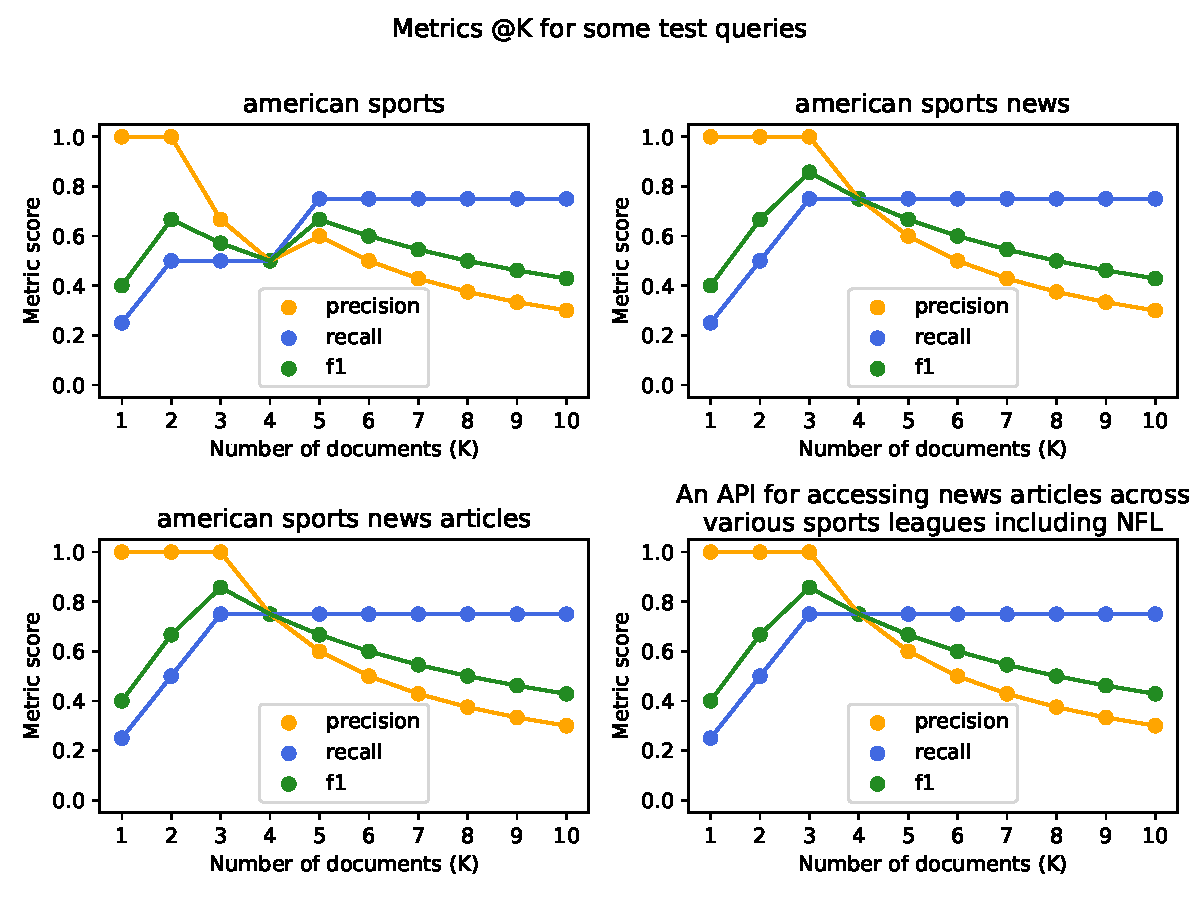
\includegraphics[width=0.8\linewidth]{assets/pdf/evaluation/prec-rec-sports}
    \end{center}

    \caption{Needles in a haystack experiment on different length queries related to American sports}
    \label{fig:nh-3}
\end{figure}

\begin{figure}[!h]
    \begin{center}
        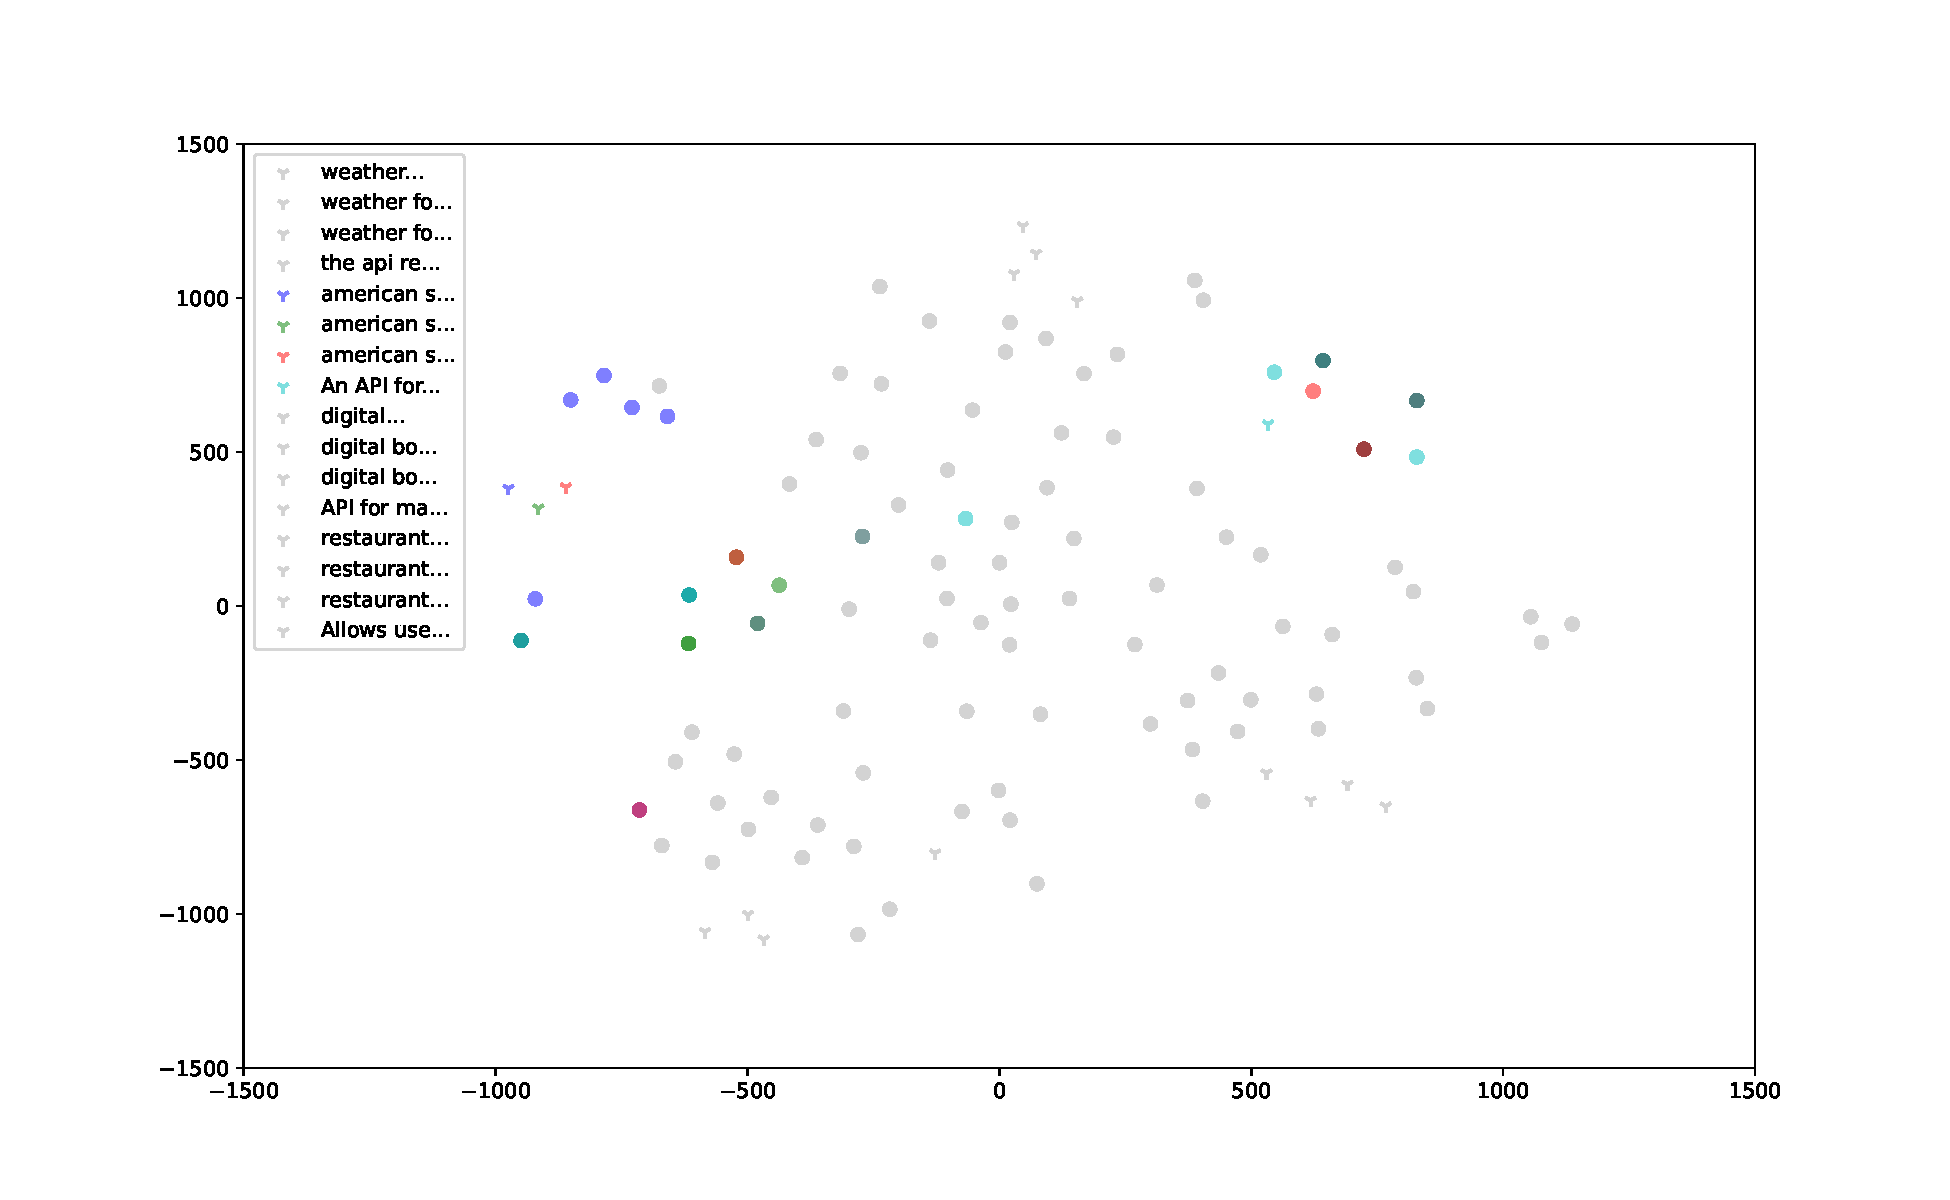
\includegraphics[width=0.8\linewidth]{assets/pdf/evaluation/tsne-sports}
    \end{center}

    \caption{t-SNE graph for the American sports queries}
    \label{fig:tsne-3}
\end{figure}

% ===========================================
% ===========================================

\begin{figure}[!h]
    \begin{center}
        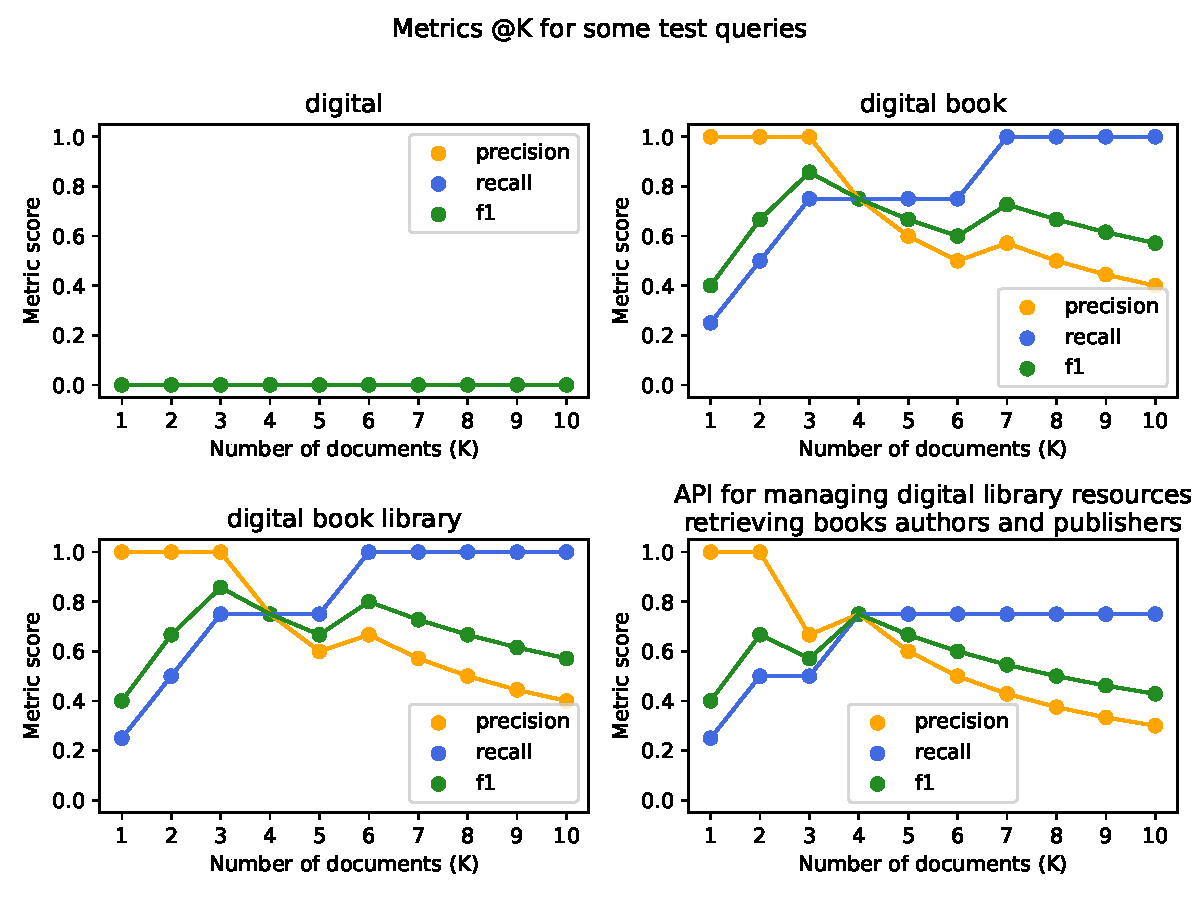
\includegraphics[width=0.8\linewidth]{assets/pdf/evaluation/prec-rec-library}
    \end{center}

    \caption{Needles in a haystack experiment on different length queries related to digital book libraries}
    \label{fig:nh-4}
\end{figure}

\begin{figure}[!h]
    \begin{center}
        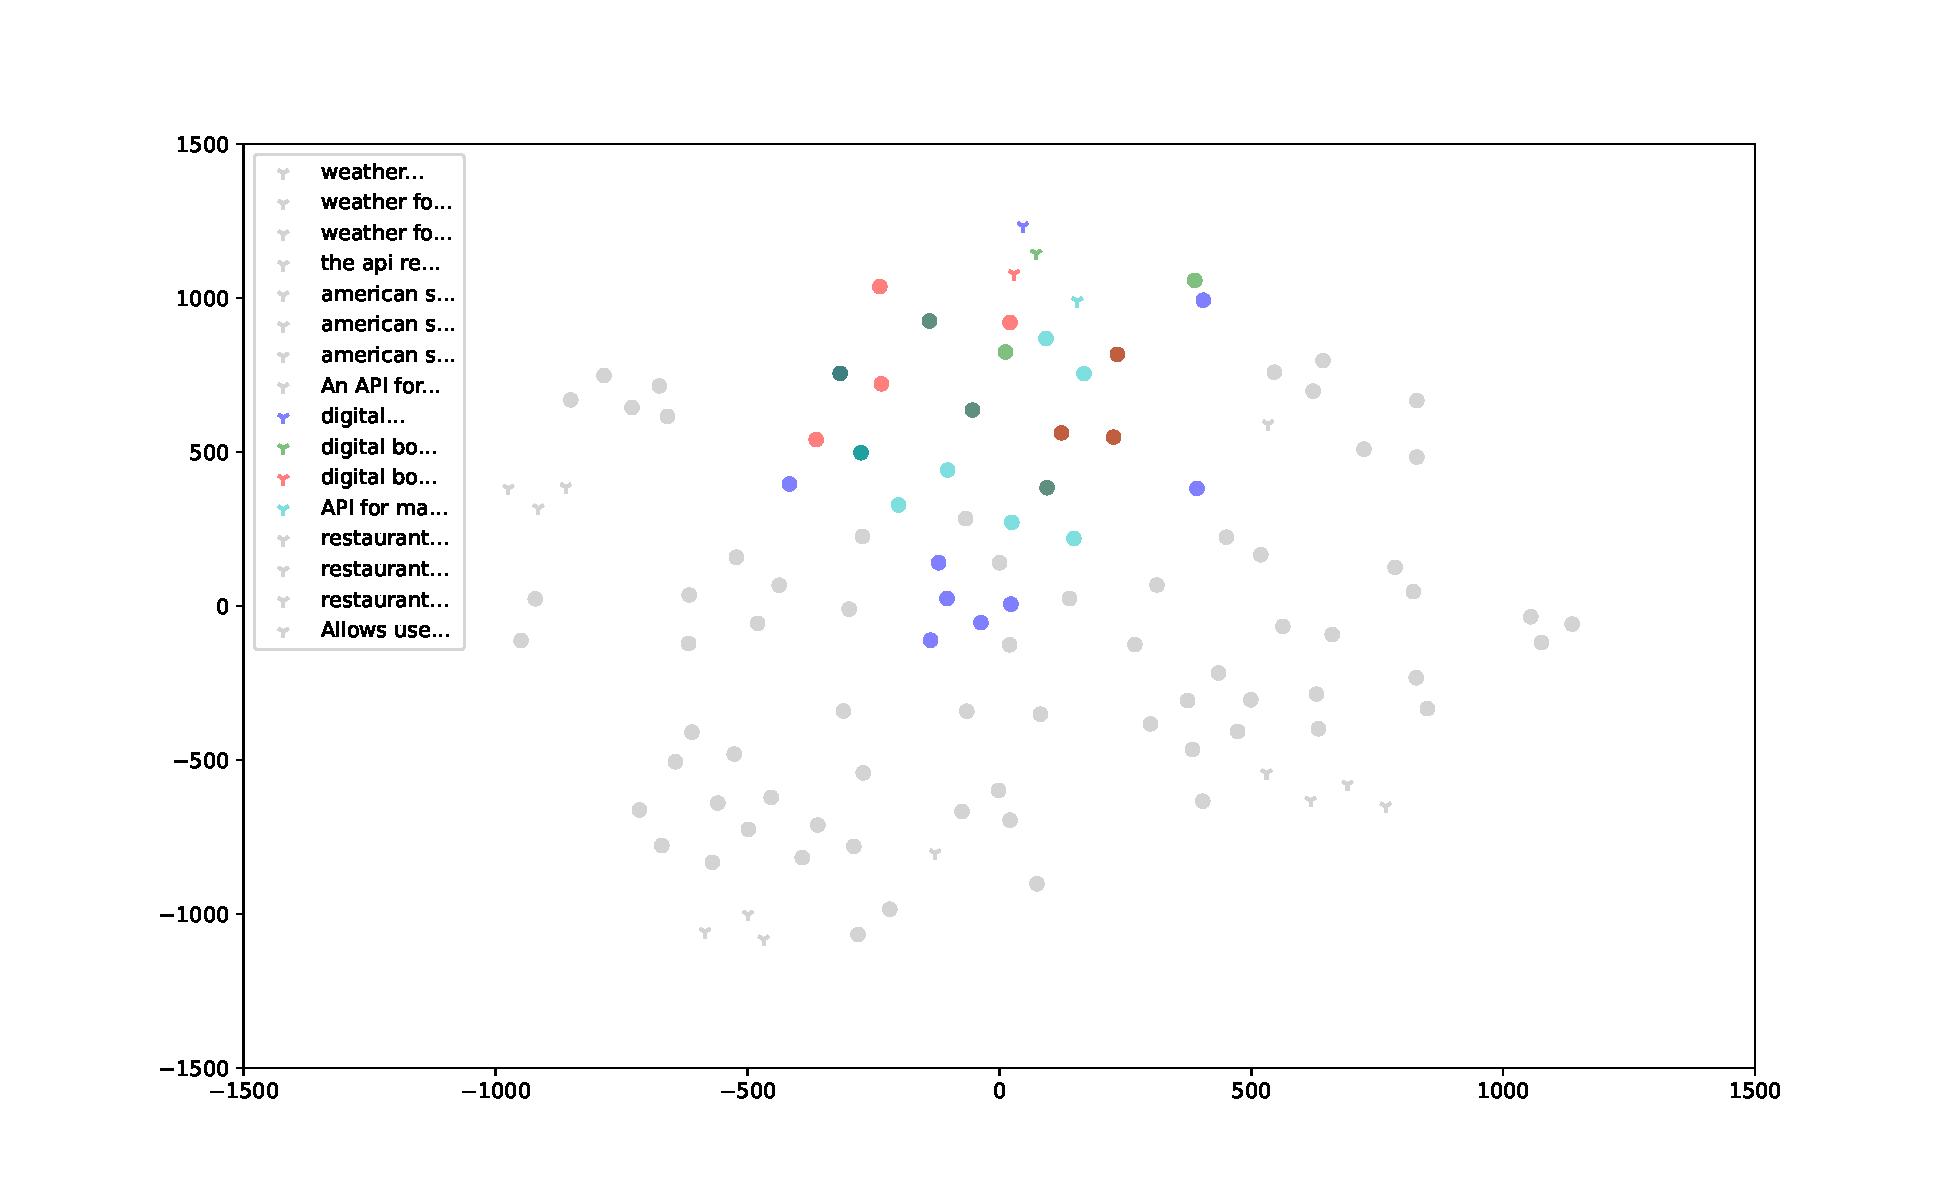
\includegraphics[width=0.8\linewidth]{assets/pdf/evaluation/tsne-books}
    \end{center}

    \caption{t-SNE graph for the digital book libraries queries}
    \label{fig:tsne-4}
\end{figure}

% ===========================================
% ===========================================

\begin{figure}[!h]
    \begin{center}
        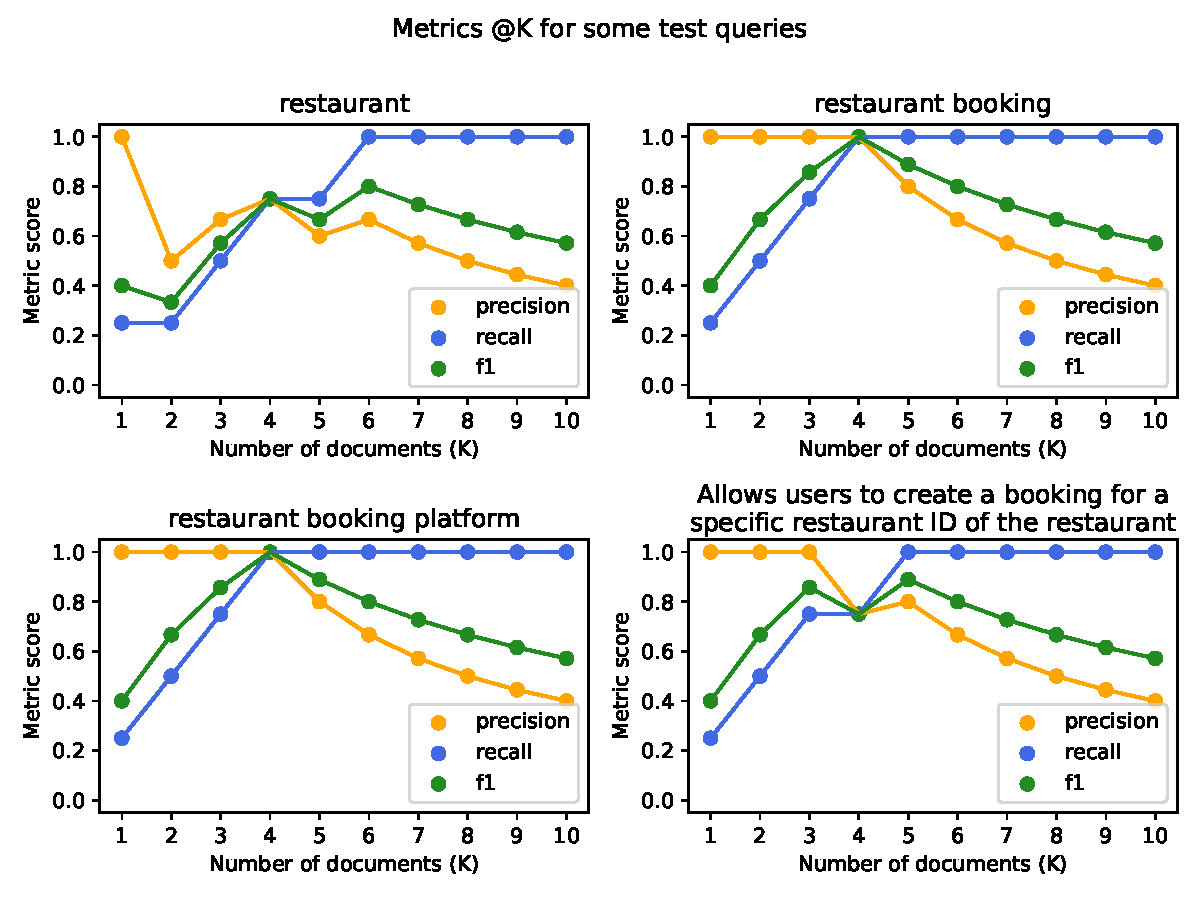
\includegraphics[width=0.8\linewidth]{assets/pdf/evaluation/prec-rec-restaurant}
    \end{center}

    \caption{Needles in a haystack experiment on different length queries related to restaurant bookings}
    \label{fig:nh-5}
\end{figure}

\begin{figure}[!h]
    \begin{center}
        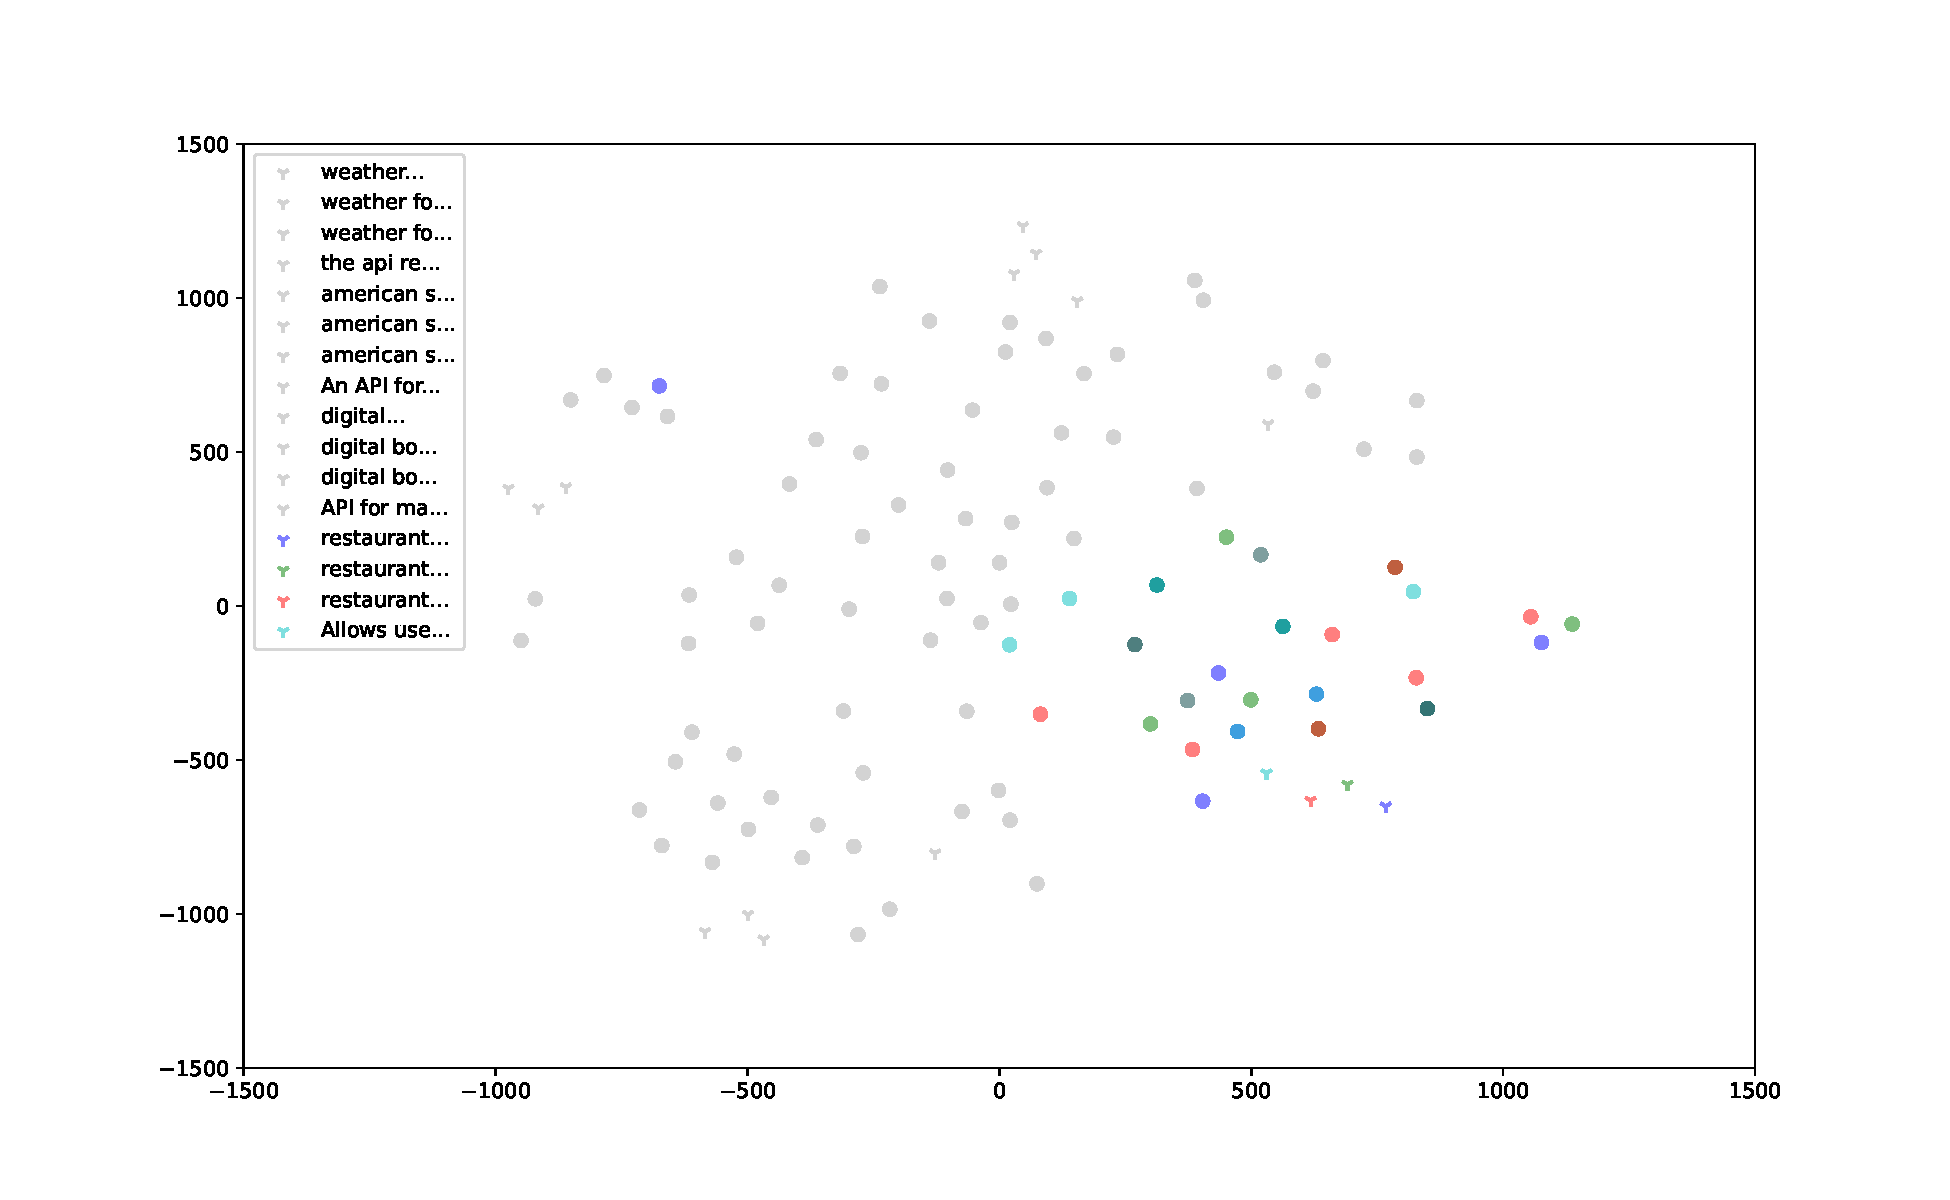
\includegraphics[width=0.8\linewidth]{assets/pdf/evaluation/tsne-restaurant}
    \end{center}

    \caption{t-SNE graph for the restaurant booking queries}
    \label{fig:tsne-5}
\end{figure}

% ===========================================
% ===========================================

\subsection{Overall Retrieval Performance}\label{subsec:overall-retrieval-performance}
In this next experiment, we used the average precision (Equation~\ref{eq:ap}) and precision to evaluate the overall performance of the system -- in this case, we are not considering the \("\)needles\("\) inserted in the previous batch of experiments. \\ \\
To compute the average precision, we need a parameter called $rel_k$ for each retrieved document.
This parameter is binary and indicates whether the document is relevant to the query or not.
Thus, for each query, we went through the first ten results and gave each one a $rel_k$ of 1 or 0.
Now that we know if a document is relevant to the query or not, we can compute the average precision at each $@K$. \\ \\
Moreover, since we now know which document is relevant and which is not, we can also compute the precision.
This is done by counting the number of relevant documents in the top ten and then dividing this number by $K$.
The results of this experiment can be found in Figure~\ref{fig:ap}.
Table~\ref{tab:metrics-pap}, instead, displays the mean average precision (Equation~\ref{eq:map}) and the overall precision for each $@K$. \\ \\
From these results, we can again build a causal graph where we have as nodes a low $K$ and a high precision.
We define a low $K$ to be $K\leq5$, while a high precision to be $P\geq0.6$.
With this causal graph, we want to see whether the first documents returned by the system are relevant or not.
As before, we use Equation~\ref{eq:prob} to compute each edge's probability.
In this case, we only need to compute the probability for path $\text{Low $K$} \rightarrow \text{High Precision}$:
\[P_1 = \frac{3}{4} = 0.75\]
The causal graph is represented in Figure~\ref{fig:dag-prec}.
In this causal graph, we can see that there is a high probability that a low value of $K$ will lead to a high precision, which is one of the main goals of a good retrieval system. \\ \\
In addition to the causal graph, in Figure~\ref{fig:es-scores}, we have plotted how the similarity score returned by Elasticsearch -- that goes from 0 to 1 -- changes for each retrieved document.
As we can see with the values for precision and average precision, the score returned by Elasticsearch drops in a similar way.

\begin{table}[!h]
    \begin{center}
        \begin{tabular}{l c c c c c c c c c c}
            \hline
            \textbf{Metric} & \textbf{@1} & \textbf{@2} & \textbf{@3} & \textbf{@4} & \textbf{@5} & \textbf{@6} & \textbf{@7} & \textbf{@8} & \textbf{@9} & \textbf{@10} \\ \hline
            $\overline{\text{Precision}}$ & 1.0 & 0.87 & 0.92 & 0.87 & 0.75 & 0.66 & 0.64 & 0.6 & 0.53 & 0.5 \\
            $\text{Mean Average Precision}$ & 1.0 & 0.81 & 0.86 & 0.78 & 0.6 & 0.42 & 0.46 & 0.4 & 0.32 & 0.27 \\ \hline
        \end{tabular}
    \end{center}

    \caption{Overall score for each metric $@K$}
    \label{tab:metrics-pap}
\end{table}

\begin{figure}[!h]
    \begin{center}
        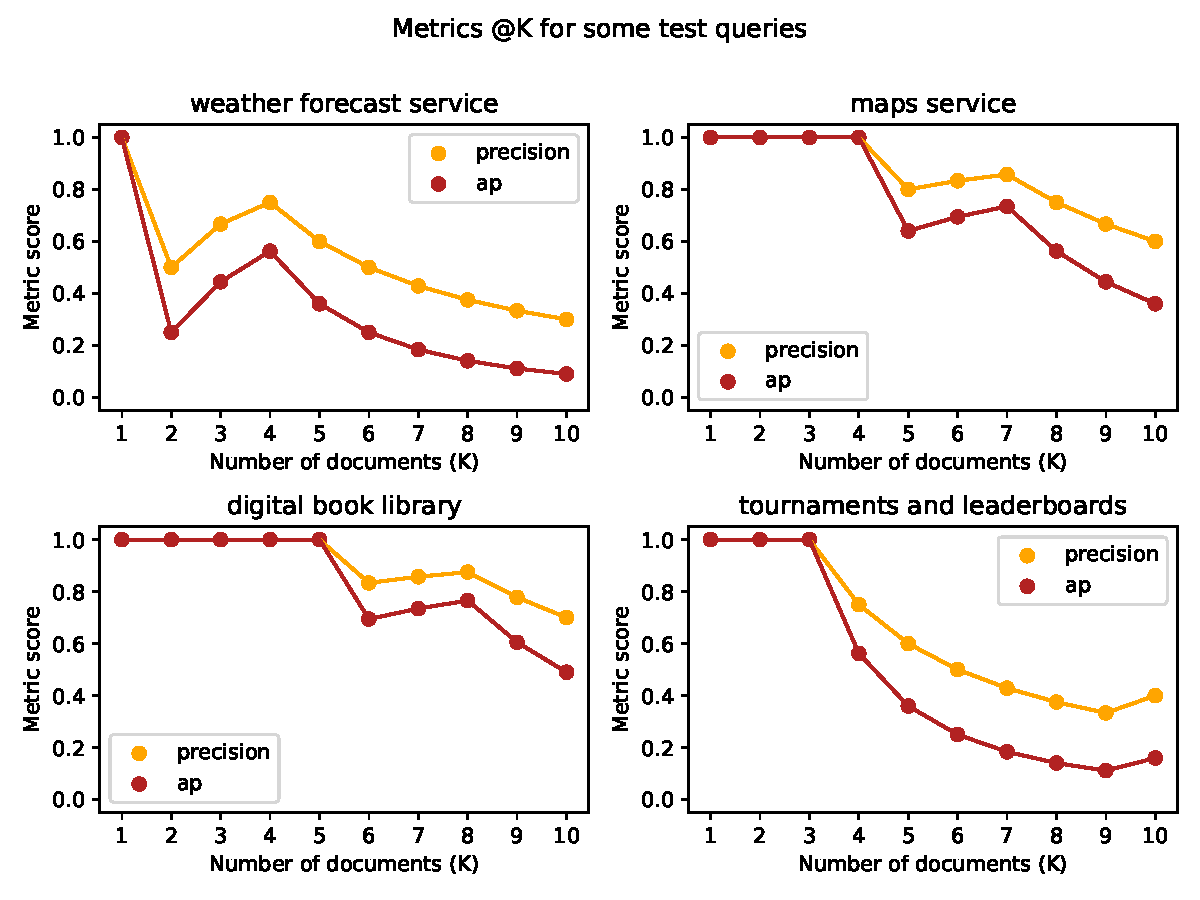
\includegraphics[width=0.8\linewidth]{assets/pdf/evaluation/ap}
    \end{center}

    \caption{Precision and Average Precision (AP)}
    \label{fig:ap}
\end{figure}

\begin{figure}[!h]
    \begin{center}
        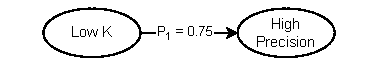
\includegraphics[width=0.4\linewidth]{assets/pdf/evaluation/dag-prec}
    \end{center}

    \caption{Causal graph with probabilities}
    \label{fig:dag-prec}
\end{figure}

\begin{figure}[!h]
    \begin{center}
        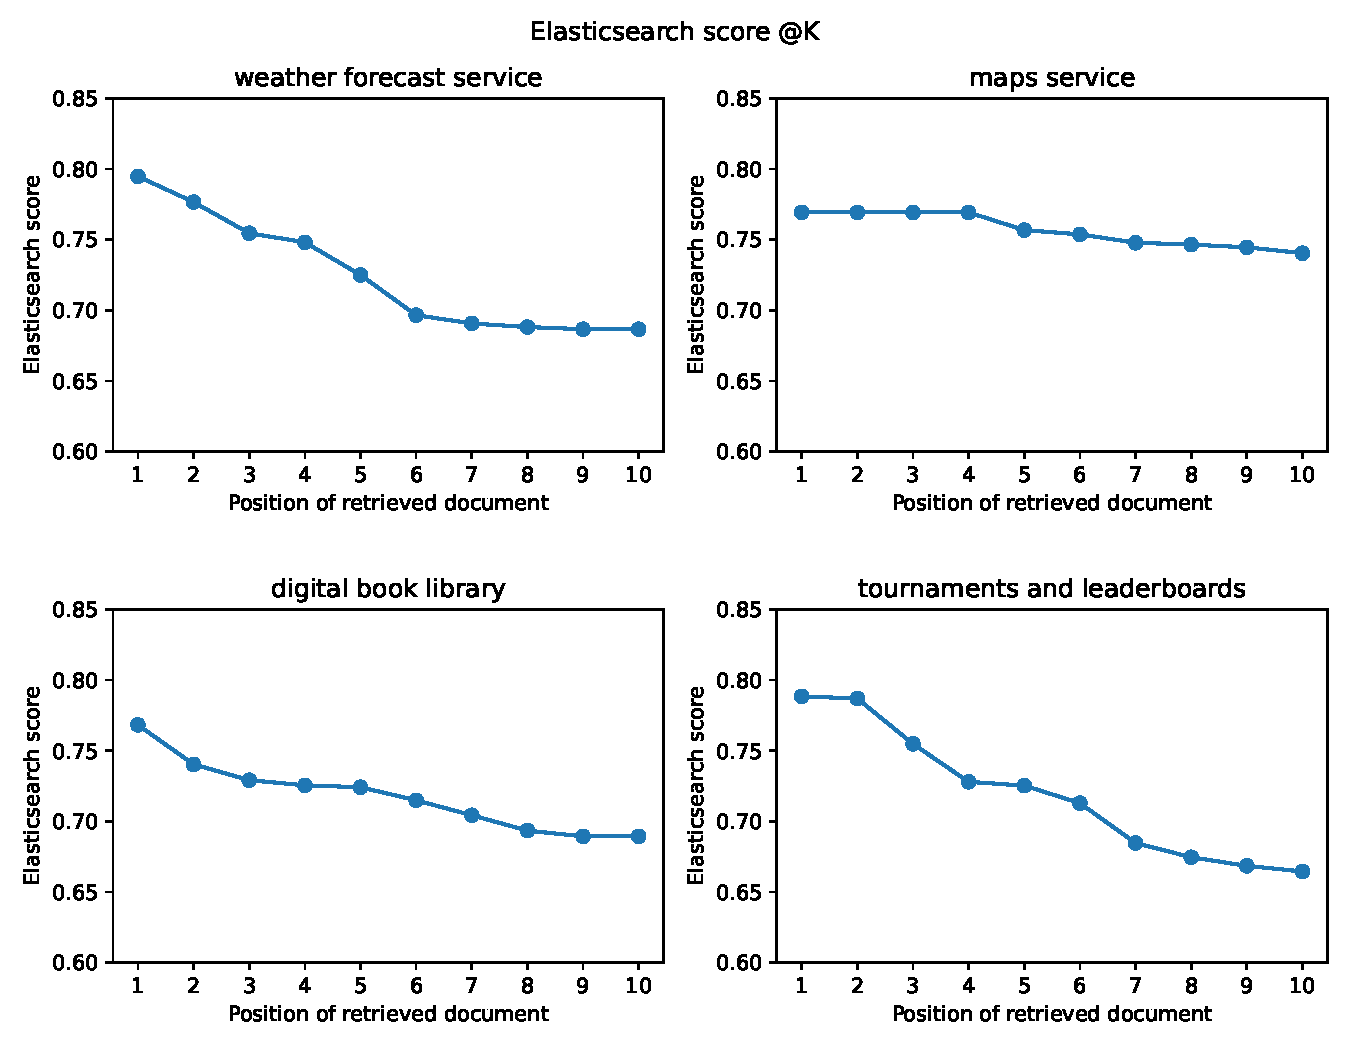
\includegraphics[width=0.8\linewidth]{assets/pdf/evaluation/es-scores}
    \end{center}

    \caption{Elasticsearch score for each retrieved document}
    \label{fig:es-scores}
\end{figure}
